% LaTeX template for creating an MNRAS paper
%
% v3.2 released 20 July 2023
% (version numbers match those of mnras.cls)
%
% Copyright (C) Royal Astronomical Society 2015
% Authors:
% Keith T. Smith (Royal Astronomical Society)

%%%%%%%%%%%%%%%%%%%%%%%%%%%%%%%%%%%%%%%%%%%%%%%%%%%%%%%%%%%%%%%%%%%%%%%%%%%%%%%%%%%%%%%%%%%%%%%%%%%%
% Basic setup. Most papers should leave these options alone.
\documentclass[fleqn,usenatbib]{mnras}

% MNRAS is set in Times font. If you don't have this installed (most LaTeX
% installations will be fine) or prefer the old Computer Modern fonts, comment
% out the following line
\usepackage{newtxtext,newtxmath}
% Depending on your LaTeX fonts installation, you might get better results with one of these:
%\usepackage{mathptmx}
%\usepackage{txfonts}

% Use vector fonts, so it zooms properly in on-screen viewing software
% Don't change these lines unless you know what you are doing
\usepackage[T1]{fontenc}

% Allow "Thomas van Noord" and "Simon de Laguarde" and alike to be sorted by "N" and "L" etc. in the bibliography.
% Write the name in the bibliography as "\VAN{Noord}{Van}{van} Noord, Thomas"
\DeclareRobustCommand{\VAN}[3]{#2}
\let\VANthebibliography\thebibliography
\def\thebibliography{\DeclareRobustCommand{\VAN}[3]{##3}\VANthebibliography}


%%%%% AUTHORS - PLACE YOUR OWN PACKAGES HERE %%%%%

% Only include extra packages if you really need them. Avoid using amssymb if newtxmath is enabled, as these packages can cause conflicts. newtxmatch covers the same math symbols while producing a consistent Times New Roman font. Common packages are:
\usepackage{graphicx}	
\usepackage{amsmath}	
\usepackage{physics}
\usepackage{enumitem}
\usepackage{anyfontsize}
\usepackage{placeins}
\usepackage{cleveref}


%%%%%%%%%%%%%%%%%%%%%%%%%%%%%%%%%%%%%%%%%%%%%%%%%%%%%%%%%%%%%%%%%%%%%%%%%%%%%%%%%%%%%%%%%%%%%%%%%%%%

%%%%% AUTHORS - PLACE YOUR OWN COMMANDS HERE %%%%%

% Please keep new commands to a minimum, and use \newcommand not \def to avoid
% overwriting existing commands. Example:
%\newcommand{\pcm}{\,cm$^{-2}$}	% per cm-squared

\graphicspath{{images/}}
%\raggedbottom               %This will let the height of the textblock vary from page to page. 

% Command to use placeins with \subsection
\makeatletter
\AtBeginDocument{%
  \expandafter\renewcommand\expandafter\subsection\expandafter
    {\expandafter\@fb@secFB\subsection}%
  \newcommand\@fb@secFB{\FloatBarrier
    \gdef\@fb@afterHHook{\@fb@topbarrier \gdef\@fb@afterHHook{}}}%
  \g@addto@macro\@afterheading{\@fb@afterHHook}%
  \gdef\@fb@afterHHook{}%
}
\makeatother

%%%%%%%%%%%%%%%%%%%%%%%%%%%%%%%%%%%%%%%%%%%%%%%%%%%%%%%%%%%%%%%%%%%%%%%%%%%%%%%%%%%%%%%%%%%%%%%%%%%%


%%%%%%%%%%%%%%%%%%% TITLE PAGE %%%%%%%%%%%%%%%%%%%%%%%%%%%%%%%%%%%%%%%%%%%%%%%%%%%%%%%%%%%%%%%%%%%%%

% Title of the paper, and the short title which is used in the headers.
% Keep the title short and informative.
\title[]{Simulating the formation of supermassive black hole binaries}

% The list of authors, and the short list which is used in the headers.
% If you need two or more lines of authors, add an extra line using \newauthor
\author[Marco Bianchi]{
Marco Bianchi
\\
% List of institutions
University of Milano-Bicocca, Physics Department, Astrophysics and Space Physics master degree\\
Dynamics of Stellar Systems 2023-2024
}

% Enter the current year, for the copyright statements etc.
\pubyear{2025}

% Don't change these lines
\begin{document}
\label{firstpage}
\pagerange{\pageref{firstpage}--\pageref{lastpage}}
\maketitle

% Abstract of the paper
\begin{abstract}
  \large The Cocoon Nebula (IC 5146) is an HII region embedded within the Barnard 168 absorption nebula, making it a prime target for studying dust extinction. 
  We obtained photometric images of IC 5146 using H$\alpha$ and H$\beta$ filters and analyzed the Balmer decrement to create a two-dimensional map of the color excess E(B-V), which serves as a proxy for dust column density. 
  Our results indicate a median E(B-V) of $\approx 0.461 \pm 0.008$ across the nebula, with a standard deviation of $\approx 0.34$. 
  A comparison with previous spectroscopic studies reveals a discrepancy in E(B-V) estimates, which we attribute to methodological differences in spatial sampling.\\
  Furthermore, given the nebula's nearly spherical morphology and its ionization by a single B0.5V-type star (BD+46 3474), we tested the Strömgren sphere model. 
  By incorporating literature values for electron density and temperature, as well as for the radius and temperature of BD+46 3474, we derived a Strömgren radius of $\approx 1.14$ pc, which is broadly consistent with the observed nebular size. 
  However, uncertainties in the nebula's distance and simplifying assumptions in the Strömgren model highlight the need for more detailed modeling.
\end{abstract} 
%%%%%%%%%%%%%%%%%%%%%%%%%%%%%%%%%%%%%%%%%%%%%%%%%%%%%%%%%%%%%%%%%%%%%%%%%%%%%%%%%%%%%%%%%%%%%%%%%%%%




%%%%%%%%%%%%%%%%% BODY OF PAPER %%%%%%%%%%%%%%%%%%%%%%%%%%%%%%%%%%%%%%%%%%%%%%%%%%%%%%%%%%%%%%%%%%%%

\section{Introduction}\label{sec:introduction}
It is a well-established fact that most galaxies host a massive black hole (MBH) at their center, with masses ranging from a few million to several billion solar masses. In the latter case, these are referred to as supermassive black holes (SMBHs).
On the other hand, galactic mergers are expected to be frequent events in the Universe, and indeed we observe many galaxies in various stages of the merging process.
This raises the question of what happens to MBHs during these mergers.
The most likely outcome is the formation of a MBH binary at the center of the newly formed galaxy.
The process leading to the formation and the evolution of such a bound state is complex and involves several stages, which were originally outlined by \cite{Begelman1980}.

\subsection{Dynamical friction}\label{sec:introduction_dynamical_friction}
In this work, we focus on the process that causes the MBHs to sink towards the core of the merger remnant, a mechanism known as \textbf{dynamical friction}.
The main idea is that a massive object moving through a stellar system will transfer energy and angular momentum to the surrounding stars, slowing down and thus spiraling inward, toward the center of mass of the system. Although the object may gain speed as it moves into a region with deeper gravitational potential, this does not contradic the previous statement, since the total orbital energy is still decreasing.
The mathematical formalization of dynamical friction was first proposed by \cite{Chandrasekhar1943}, based on the assumption that the stellar background is homogeneous and isotropic.
In particular, the perturber is subject to a deceleration given by the following equation:
{\fontsize{8.5pt}{8.5pt}\begin{equation}
    \dfrac{d\vec{v}_M}{dt} \, = \, -16 \pi^2 G^2 m \left(m+M\right) \ln \Lambda \left[\int^{v_M}_0 f(v_m) v_m^2 dv_m\right] \dfrac{\vec{v}_M}{v_M^3},
    \label{eq:chandrasekhar}
\end{equation}}
where $\ln \Lambda$ is the Coulomb logarithm (which depends on the maximum and minimum impact parameters of the interaction), $m$ is the mass of the background particles, $M$ is the mass of the perturber, and $f(v_m)$ is the distribution function of the background particles.
Dynamical friction is most efficient when $v_M \simeq v_m$, which is typically the case during the inspiral, and becomes negligible for $v_M \ll v_m$ or $v_M \gg v_m$.

Once the MBHs have sunk to the center of the merger remnant and their separation is such that each is primarily influenced by the gravitational pull of the other, they form a bound state.
The critical separation at which this occurs can be approximated by the \textbf{influence radius}, i.e., the distance at which the gravitational potential energy of the MBH is comparable to the kinetic energy of the surrounding stars:
{\fontsize{7.4pt}{7.4pt}\begin{equation}
    r_\text{inf} = \dfrac{GM}{\sigma^2} 
    \approx 1 \left(\dfrac{M}{10^6 M_\odot}\right) \left(\dfrac{\sigma}{70 \text{km/s}}\right)^{-2} \text{pc} 
    \approx 50 \left(\dfrac{M}{10^9 M_\odot}\right) \left(\dfrac{\sigma}{300 \text{km/s}}\right)^{-2} \text{pc} ,
    \label{eq:influence_radius}
\end{equation}}
where $\sigma$ is the velocity dispersion of the stars surrounding the MBH.

The formation of the binary causes a sudden change in the velocities of the MBHs relative to the surrounding stars, making dynamical friction inefficient.
Morever, once the MBHs are bound, dynamical friction acts of the center of mass of the binary, rather than on the individual MBHs.

The next step is to determine whether other mechanisms can reduce the binary separation further, eventually leading to coalescence.
It is well known that compact-object binaries lose energy and angular momentum via gravitational waves emission, thus shrinking their orbits.
However, this process becomes efficient only when the binary separation is already very small, of the order of a few milliparsecs.
We therefore need to identify a mechanism capable of bridging the gap from parsecs to milliparsecs.
This is the so-called \textbf{final-parsec problem}, which has been the subject of extensive research in the past decades.
The most promising solution is \textbf{stellar hardening}, a process in which stars undergo three-body interactions with the binary, extracting energy and angular momentum from it.
More informations on this process can be found in \cite{Quinlan1996}.
%%%%%%%%%%%%%%%%%%%%%%%%%%%%%%%%%%%%%%%%%%%%%%%%%%

\subsection{Modeling galactic bulges with Barnes' treecode}\label{sec:introduction_models}
The efficiency of dynamical friction depends on the density and velocity distribution of the stars that constitute the bulge of the merger remnant.
This is typically modeled as a spherically symmetric distribution of particles, with a density profile that decays with distance from the center.
The model most commonly used in analytical calculations is the \textbf{singular isothermal sphere} (SIS), whose density and mass profiles are given by:
\begin{equation}
    \rho_\text{SIS}(r) = \dfrac{\sigma^2}{2 \pi G r^2} \:\: , \:\: M_\text{SIS}(r) = \dfrac{2 \sigma^2}{G} r \:\:.
    \label{eq:sis_density}
\end{equation}
However, this model is not realistic, as it diverges at $r=0$ and predicts an infinite total mass.
In the next section, we will introduce more physical alternatives that remain spherically symmetric but possess finite total mass.

In any case, modeling a galactic bulge requires a large number of particles, typically of the order of $N \approx 10^6$.
Therefore, the use of direct N-body simulations — which have a computational complexity of $\mathcal{O}(N^2)$ — is not feasible.
Instead, a \textbf{treecode} algorithm allows to approximate the gravitational potential of a system of particles by organizing them into a hierarchical tree structure.
If the size of a cell — as seen from the point where the force is being computed — is sufficiently small, the group can be treated as a single particle, thus reducing the number of pairwise interactions to $\mathcal{O}(N \log N)$.
In particular, we will use the treecode developed by \cite{Barnes1986}, which is a well-known implementation of this algorithm.
It allows the user to set the following parameters:
\begin{itemize}[wide, labelwidth=!, itemindent=!, labelindent=0pt, itemsep=0.1em]
  \item \textbf{Integration time-step $dt$:} the time interval between two consecutive updates of particle positions and velocities. It must be small enough to ensure accurate integration of the system's evolution, but large enough to keep the computational time manageable. 
  \item \textbf{Opening angle $\theta$:} determines the accuracy of the treecode approximation by controlling how small the angle subtended by a cell must be before it can be treated as a single particle.
  \item \textbf{Softening radius $\epsilon$:} gravitational forces are smoothed by replacing each particle with a Plummer sphere of scale length $\epsilon$, preventing the force from diverging at small distances and producing non-physical interactions. 
\end{itemize}
%%%%%%%%%%%%%%%%%%%%%%%%%%%%%%%%%%%%%%%%%%%%%%%%%%
%%%%%%%%%%%%%%%%%%%%%%%%%%%%%%%%%%%%%%%%%%%%%%%%%%%%%%%%%%%%%%%%%%%%%%%%%%%%%%%%%%%%%%%%%%%%%%%%%%%%


\section{Distributing particles according to three models}\label{sec:observation}
As we introduced in the previous section, the SIS density profile of Eq. \ref{eq:sis_density} is not physical, as it diverges at $r=0$ and has an infinite total mass.
Therefore, a realistic density profile must have a finite central value and decrease faster than $r^{-3}$ at large distances.
In this section, we will start with a naive regularization of the SIS model, and then we will introduce two more realistic models that are commonly used to describe the density distribution of galactic bulges.
For each model, we will derive the radial probability distribution function (PDF) of the particles, which can be used to sample their positions.
\vspace{0.5em}

For every spherically symmetric model, the angular PDFs of the particles are given by:
\begin{equation}
    p(\phi) = \dfrac{1}{2 \pi} \:\: \text{and} \:\: p(\theta) = \dfrac{\sin \theta}{2}  \:\: ,
    \label{eq:angular_pdf}
\end{equation}
which can be easily integrated to obtain the cumulative distribution functions (CDFs).
The \textbf{direct Monte Carlo sampling method} allows to sample each angle simply by generating CDF samples $P \in [0,1]$ from a uniform distribution and then inverting the CDF formula:
\begin{equation}
    \phi(P_\phi) = 2 \pi P_\phi \:\: , \:\: \theta(P_\theta) = \arccos\left(1 - 2 P_\theta\right) \:\: .
    \label{eq:angular_sampling}
\end{equation}

\subsection{Regularized isothermal sphere}\label{sec:isothermal_sphere}
The first model we will consider is a regularized version of the SIS, which we will refer to as the \textbf{regularized isothermal sphere} (RIS).
The idea is to cure the divergence at $r=0$ by introducing a softening radius $r_0$ (which has nothing to do with that used in the treecode).
We also add an exponential cutoff at large distances, governed by a scale length $R$.
The resulting density profile is given by:
\begin{equation}
    \rho_\text{RIS}(r) = \dfrac{\sigma^2}{2 \pi G \left(r + r_0\right)^2} e^{-r/R} \:\: .
    \label{eq:ris_density}
\end{equation}
Given the density profile, we can easily compute the radial PDF of the particles, which is given by:
\begin{equation}
    p_\text{RIS}(r)dr = \dfrac{4\pi r^2 \rho_\text{RIS}(r)}{M_\text{tot}} dr \propto \dfrac{r^2 e^{-r/R}}{\left(r + r_0\right)^2} dr\:\: .
    \label{eq:ris_pdf}
\end{equation}
Integrating $p_\text{RIS}(r)$ to obtain the CDF is not trivial, let alone inverting it to obtain the sampling formula.
However, we can use the \textbf{acceptance-rejection sampling method} to generate samples from the PDF, using a decreasing exponential function as the proposal distribution.
This procedure, together with the angular sampling of Eq. \ref{eq:angular_sampling}, allows us to sample particle positions from the RIS model.
\vspace{0.5em}

In order to evolve the system, we need to assign an initial velocity to each particle.
In general, this should be achieved by sampling from the conditional velocity PDF at radius $r$, which is given by
\begin{equation}
    p(v|r)dv = \dfrac{f(\mathcal{E}(v|r))}{n(r)} v^2 dv \:\: ,
    \label{eq:velocity_pdf}
\end{equation}
where $n(r)$ is the number density of particles at radius $r$ and $f(\mathcal{E}(r,v))$ is the distribution function of the particles per unit of phase-space volume.
Given $\rho(r)$, we could derive the gravitational potential $\phi(r)$ by solving the Poisson equation and then the distribution function $f(\mathcal{E}(r,v))$ by solving the Eddington equation.
Nonetheless, this is a complex task that is beyond the scope of this naive model.
Therefore, we approximate the distribution function of the RIS model with that of the SIS model, which is a three-dimensional Maxwellian distribution with dispersion $\sigma$:
\begin{equation}
    p_\text{SIS}(v|r)dv \propto e^{-\frac{v^2}{2 \sigma^2}} v^2 dv \propto 
    \prod_{i=x,y,z} e^{-\frac{v_i^2}{2 \sigma^2}} v_i^2 dv_i \:\: .
    \label{eq:sis_distribution_function}
\end{equation}
To determine the value of $\sigma$, we impose the virial theorem:
\begin{equation}
    \sum_{j > i} - \dfrac{G m_i m_j}{r_{ij}} = E_\text{grav,tot} = -2E_\text{kin,tot} \simeq -2\dfrac{1}{2} N m v^2 \simeq -3 N m \sigma^2 \:\:. 
    \label{eq:sigma_virial}
\end{equation}

%%%%%%%%%%%%%%%%%%%%%%%%%%%%%%%%%%%%%%%%%%%%%%%%%%

\subsection{King model}\label{sec:King_model}

%%%%%%%%%%%%%%%%%%%%%%%%%%%%%%%%%%%%%%%%%%%%%%%%%%

\subsection{Hernquist model}\label{sec:Hernquist_model}
\begin{figure}\centering
	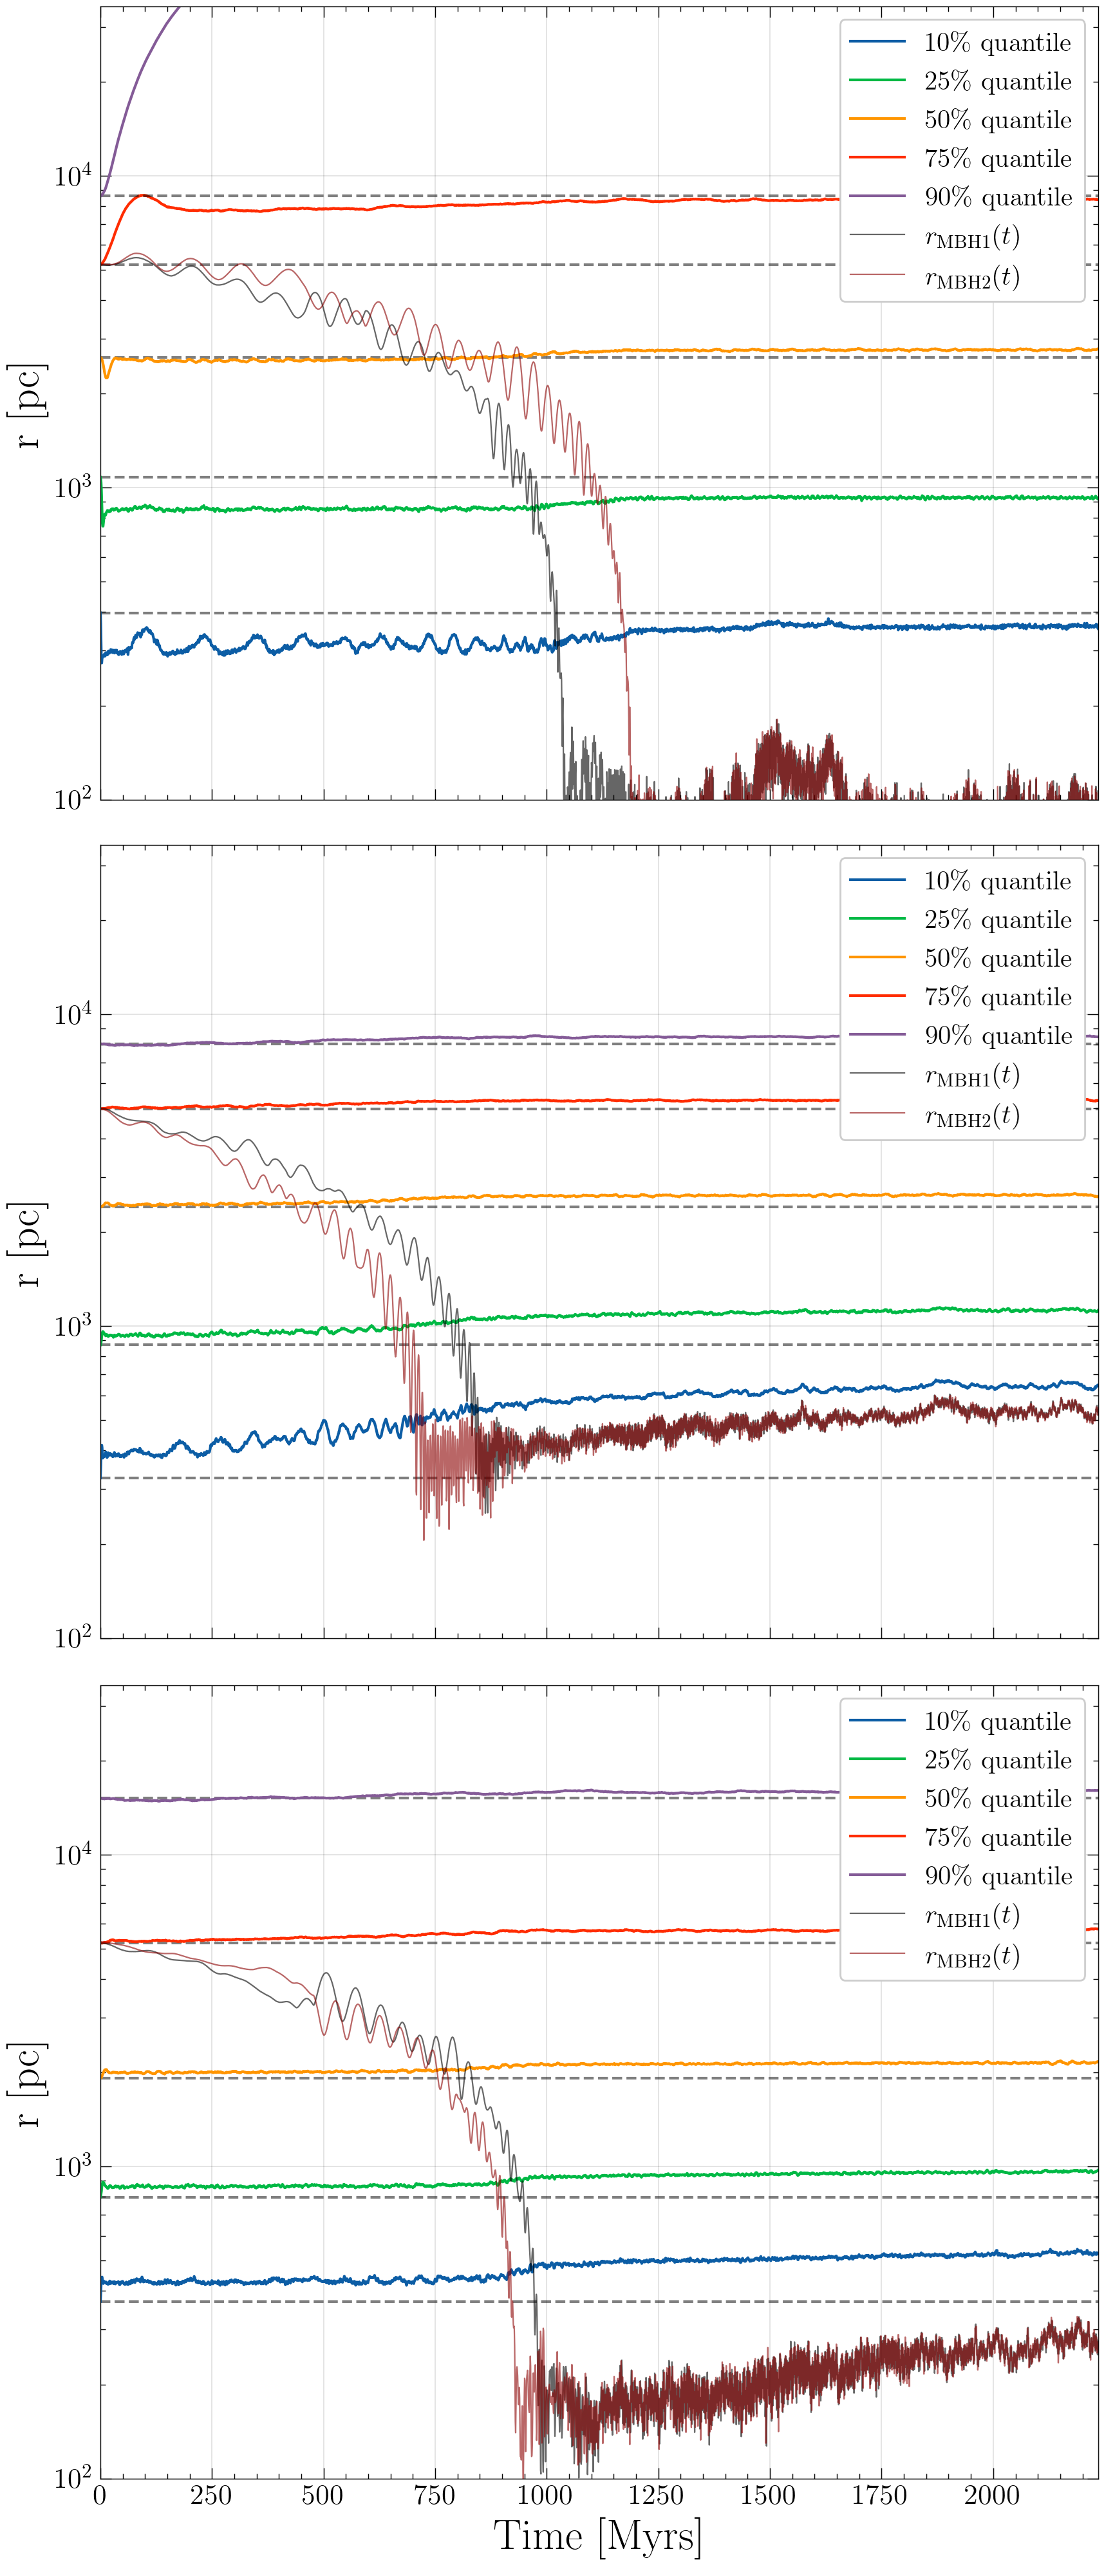
\includegraphics[width=1.\columnwidth]{LR_50K_dt0005.png}
    \caption{Lagrangian radii of the regularized isothermal sphere (upper panel), King distribution (central panel), and Hernquist distribution (lower panel). The MBHs' positions are also shown.}
    \label{fig:Lagrangian_radii}
\end{figure}
%%%%%%%%%%%%%%%%%%%%%%%%%%%%%%%%%%%%%%%%%%%%%%%%%%
%%%%%%%%%%%%%%%%%%%%%%%%%%%%%%%%%%%%%%%%%%%%%%%%%%%%%%%%%%%%%%%%%%%%%%%%%%%%%%%%%%%%%%%%%%%%%%%%%%%%


\section{Simulation}\label{sec:simulation}
We chose $dt = 0.0005 \,\text{iu} \approx 7.5 \times 10^4 \,yr$. We chose $\theta=0.3$. We chose $\epsilon=0.1 \,\text{iu} = 100 \,\text{pc}$.
%%%%%%%%%%%%%%%%%%%%%%%%%%%%%%%%%%%%%%%%%%%%%%%%%%
%%%%%%%%%%%%%%%%%%%%%%%%%%%%%%%%%%%%%%%%%%%%%%%%%%%%%%%%%%%%%%%%%%%%%%%%%%%%%%%%%%%%%%%%%%%%%%%%%%%%



\section{Conclusion}\label{sec:conclusion}
%%%%%%%%%%%%%%%%%%%%%%%%%%%%%%%%%%%%%%%%%%%%%%%%%%
%%%%%%%%%%%%%%%%%%%%%%%%%%%%%%%%%%%%%%%%%%%%%%%%%%%%%%%%%%%%%%%%%%%%%%%%%%%%%%%%%%%%%%%%%%%%%%%%%%%%


%%%%%%%%%%%%%%%%%%%% REFERENCES %%%%%%%%%%%%%%%%%%%%%%%%%%%%%%%%%%%%%%%%%%%%%%%%%%%%%%%%%%%%%%%%%%%%
% The best way to enter references is to use BibTeX:
\bibliographystyle{mnras}
\bibliography{bibliography} 
%%%%%%%%%%%%%%%%%%%%%%%%%%%%%%%%%%%%%%%%%%%%%%%%%%%%%%%%%%%%%%%%%%%%%%%%%%%%%%%%%%%%%%%%%%%%%%%%%%%%


% Don't change these lines
\label{lastpage}
\end{document}
